\section{Entwicklung eines Konzepts für die Verifizierung und das Labeln der Ereignisse} \label{sec:Meth Labeling}
Da die Modellauswahl eingegrenzt wurde auf Modelle des überwachten Lernens, werden gelabelte Ereignisse benötigt. Dafür ist ein Konzept zu erstellen. Grundlage für das Labeln ist ein Datensatz mit herausgesuchten Ereignissen. Das Sammeln erfolgte bereits vor dieser Arbeit. Diese herausgesuchten Ereignisse sind mit einem Label, einem Datum, der Startuhrzeit und der Enduhrzeit des Ereignisses vermerkt. Die Uhrzeiten sind jedoch nur grob ermittelt. Die Ereignisse sind in einer csv-Datei gespeichert. Genaueres zu diesem Datensatz folgt in  \autoref{sec:Meth Datensatz}. \par

Es ist wichtig, dass ein Ereignis zeitlich exakt eingegrenzt wird, damit die charakteristischen Merkmale daraus extrahiert werden können. Ebenfalls soll sichergestellt werden, dass in einem angegebenen Zeitraum auch genau diese charakteristischen Merkmale zu sehen sind. Aus diesem Grund sind die herausgesuchten Ereignisse zu verifizieren und der exakte Zeitraum ist zu bestimmen. \par 

Die Verifizierung erfolgt visuell. Dafür werden die Videos benötigt, in denen ein Ereignis dargestellt sein muss. Der exakte Start- und Endzeitpunkt eines Ereignisses muss markiert werden können. Dazu können die Detektionsdatensätze verwendet werden (\autoref{sec:Meth RohDat}). In diesen ist für jedes Frame ein Zeitstempel sowie eine Identifikationsnummer jedes Frame vorhanden. Die Identifikationsnummer stimmt mit der Position des Frames im Video überein. Darüber lassen sich die Frames und die Datensatzeinträge zuordnen. Das Verifizierungsprogramm bekommt somit als Eingabe die Liste mit den herausgesuchten Ereignissen, die Videos und die  Detektionsdatensätze. Die Suche nach den Videos und Detektionsdatensätzen wird von einem Hilfsmodul übernommen. Dieses sucht basierend auf Datums- und Zeitpunktangaben die Dateipfade heraus. Das Programm erstellt einen Datensatz mit den verifizierten Ereignissen. In diesem ist das Label des Ereignisses, der exakte Startzeitpunkt und der Endzeitpunkt vermerkt. Ebenfalls gibt das Programm aus, welche Ereignissen sich nicht verifizieren ließen. Die Detektionsdaten müssen aus der Datenbank in eine csv-Datei heruntergeladen werden. Ist dies noch nicht erfolgt, kann ein Ereignis nicht verifiziert werden. Ereignisse mit fehlenden Detektionsdaten oder Videos werden ebenfalls in einer Liste vermerkt. Diese Liste kann von einem weiteren Programm gelesen werden, das versucht, die fehlenden Daten herunterzuladen. Anschließend kann erneut versucht werden, das Ereignis zu verifizieren. Final erstellt das Programm eine Liste mit allen Ereignissen, die sich verifizieren ließen. Das Blockdiagramm dieses Konzepts ist in der Abbildung \ref{fig:BlockLabeling} zu sehen. 

\begin{figure}[htbp]
    \centering
    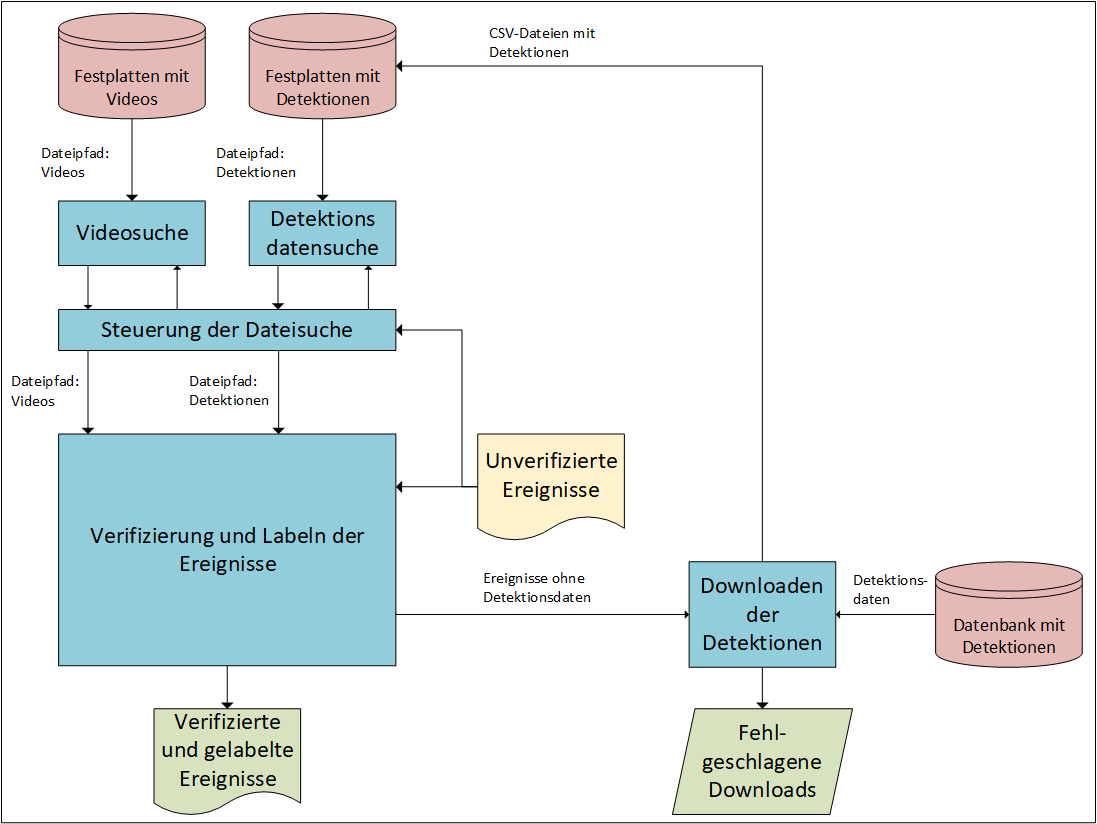
\includegraphics[width=\textwidth]{img/Grafiken/Verifizierungstool Konzept.png}
    \caption[Blockdiagramm des Verifizierungskonzepts.]{Blockdiagramm des Verifizierungskonzepts. Blau dargestellt sind die Programmmodule. Die Eingänge sind Gelb markiert, Ausgänge sind Grün und Speicher sind Rot abgebildet.}
    \label{fig:BlockLabeling}
\end{figure}


Wie erwähnt, muss die Verifizierung visuell über die Videos erfolgen. Ideal ist es, wenn der Anwender direkt im Video die Zeitpunkte eines Ereignisses markieren kann. Dies ist über den folgenden Weg möglich. Der Anwender schaut sich das Video an, findet er das zu verifizierende Ereignis, wählt er ein Frame als Startframe aus. Über die Position des Frames im Videowird seine Identifikationsnummer ermittelt. Mit dieser wird der zugehörige Eintrag im Detektionsdatensatz gesucht. Dort ist der Zeitstempel vermerkt. Der Zeitstempel wird als Startzeitpunkt abgespeichert. \par 

Anwenderfreundlich ist auch eine Automatisierung des Prozesses, sodass nicht jedes Ereignis, das zugehörige Video und die Detektionsdaten manuell ausgewählt und herausgesucht werden müssen. Für das Heraussuchen der Videos und der Detektionsdatensätze wurden bereits vor dieser Arbeit Programme geschrieben, die dies automatisieren. Lediglich ein Datum und ein Zeitpunkt werden benötigt, um die entsprechenden Dateien herauszusuchen. Da die Ereignisse in einer csv-Datei abgelegt sind, können diese iterativ aufgerufen werden. So ist der gesamte Ablauf automatisierbar. \par

Das Programm zum Herunterladen der Detektionsdaten entstand ebenfalls bereits vor dieser Arbeit und ließ sich leicht in das Konzept integrieren. 